\documentclass[border=10pt]{standalone}
\usepackage[svgnames]{xcolor}
\usepackage{amsmath}
\usepackage{pgfplots}
\pgfplotsset{compat=newest}
\usepackage[sfdefault]{FiraSans}
\usepackage{FiraMono}
\renewcommand*\familydefault{\sfdefault}
\begin{document}
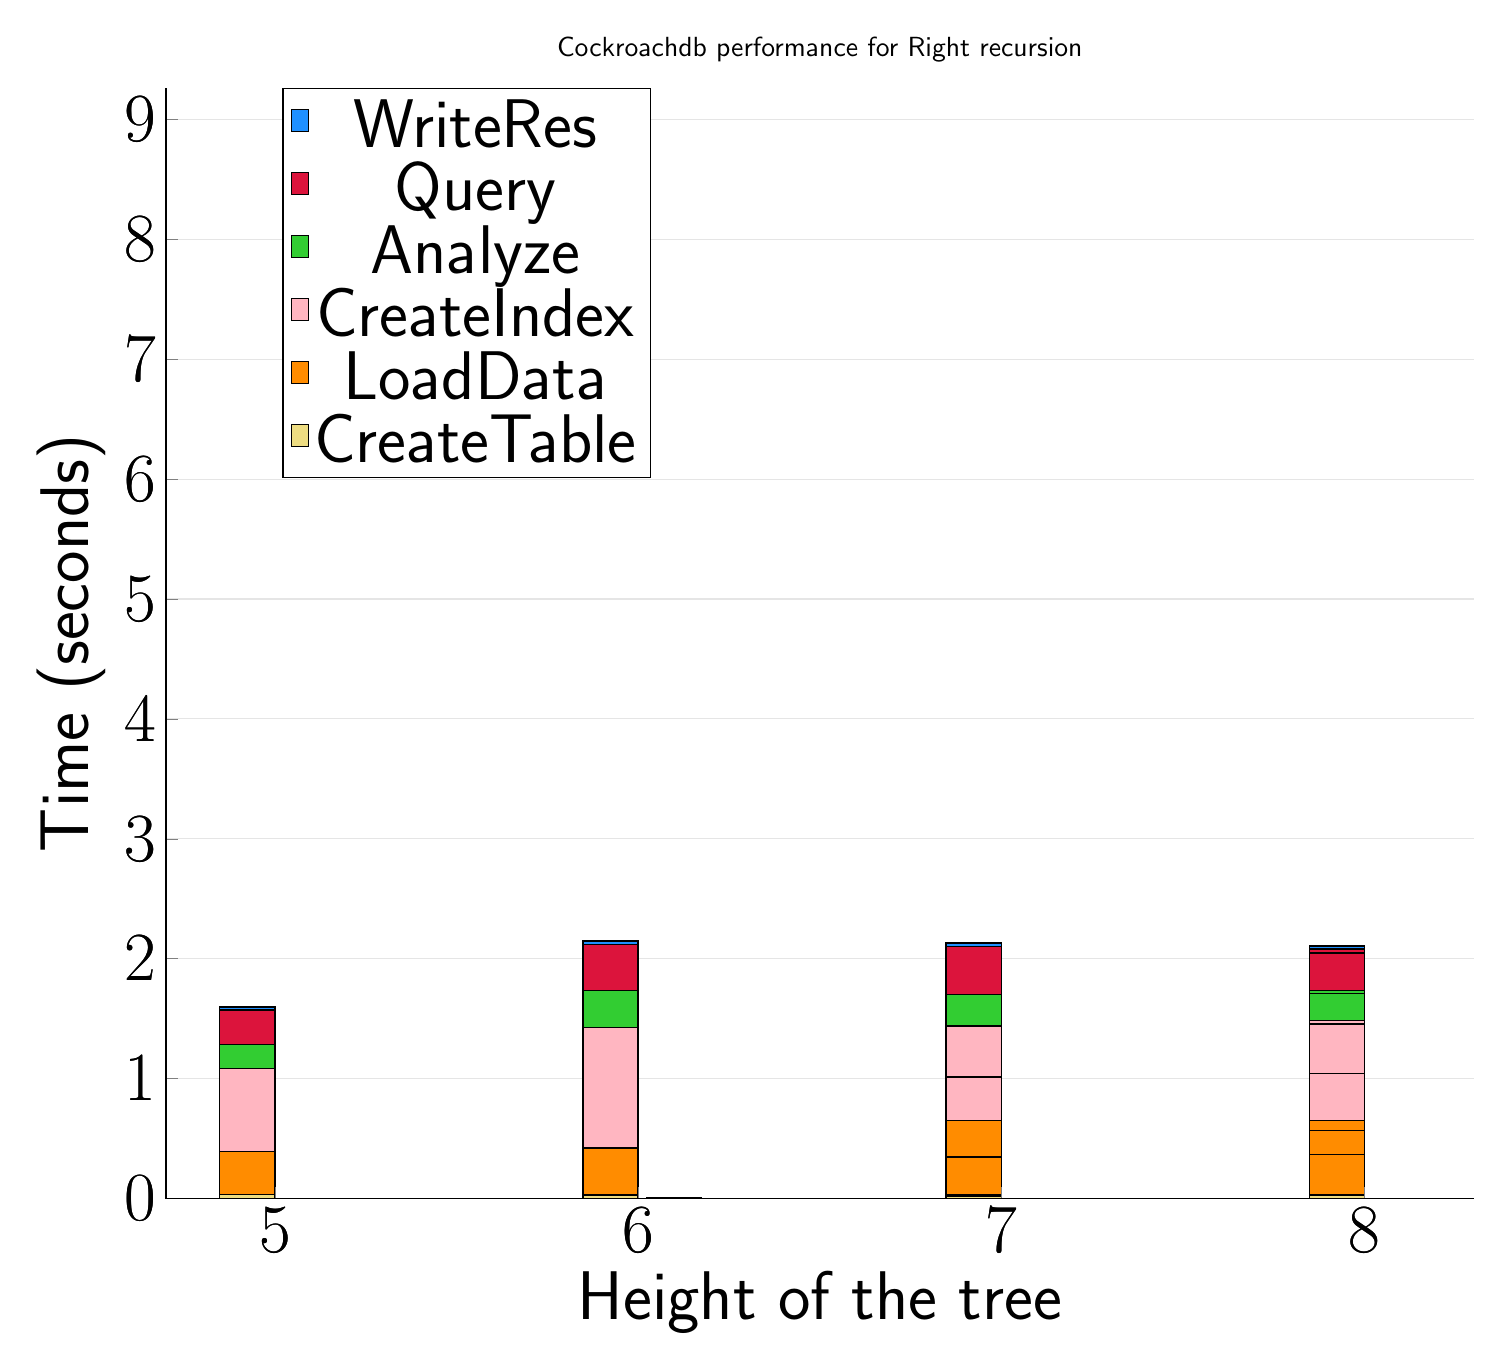
\begin{tikzpicture}
\begin{axis}[
   ybar stacked,
   title={Cockroachdb performance for Right recursion},
   bar shift=-10pt,
   width=1.5\textwidth,
   bar width=0.7cm,
   ymajorgrids, tick align=inside,
   major grid style={draw=gray!20},
   xtick=data,
   ymin=0, ymax=9.263333335518837,
   axis x line*=bottom,
   axis y line*=left,
   enlarge x limits=0.1,
   legend style={
       at={(0.23, 1)},
       anchor=north,
       legend columns=1,
       font=\Huge,
   },
   ylabel={Time (seconds)},
   xlabel={Height of the tree},
   label style={font=\Huge},
   tick label style={font=\Huge},
]
\addlegendimage{fill=DodgerBlue, draw=black, line width=0.2pt}
\addlegendentry{WriteRes}
\addlegendimage{fill=Crimson, draw=black, line width=0.2pt}
\addlegendentry{Query}
\addlegendimage{fill=LimeGreen, draw=black, line width=0.2pt}
\addlegendentry{Analyze}
\addlegendimage{fill=LightPink, draw=black, line width=0.2pt}
\addlegendentry{CreateIndex}
\addlegendimage{fill=DarkOrange, draw=black, line width=0.2pt}
\addlegendentry{LoadData}
\addlegendimage{fill=LightGoldenrod, draw=black, line width=0.2pt}
\addlegendentry{CreateTable}
\addplot +[fill=LightGoldenrod, draw=black, line width=0.5pt] coordinates {
    (5, 0.03333333134651184)
    (6, 0.02999999870856603)
    (7, 0.02666666607062022)
    (7, 0.019999998311201733)
    (7, 0.033333333830038704)
    (8, 0.023333335916201275)
    (8, 0.033333333830038704)
    (8, 0.03333332886298498)
};
\addplot +[fill=DarkOrange, draw=black, line width=0.5pt] coordinates {
    (5, 0.3566666692495346)
    (6, 0.39000000307957333)
    (7, 0.6266666650772095)
    (7, 0.3266666655739148)
    (7, 0.3133333350221316)
    (8, 0.34333333373069763)
    (8, 0.6199999998013178)
    (8, 0.5366666639844576)
};
\addplot +[fill=LightPink, draw=black, line width=0.5pt] coordinates {
    (5, 0.6933333352208138)
    (6, 1.0066666677594185)
    (7, 0.7866666664679846)
    (7, 0.663333331545194)
    (7, 0.6733333319425583)
    (8, 0.676666667064031)
    (8, 0.8299999982118607)
    (8, 0.8866666679581007)
};
\addplot +[fill=LimeGreen, draw=black, line width=0.5pt] coordinates {
    (5, 0.20333333065112433)
    (6, 0.3099999974171321)
    (7, 0.2600000003973643)
    (7, 0.20000000298023224)
    (7, 0.20666666825612387)
    (8, 0.20333333313465118)
    (8, 0.25333333512147266)
    (8, 0.25333333263794583)
};
\addplot +[fill=Crimson, draw=black, line width=0.5pt] coordinates {
    (5, 0.2866666664679845)
    (6, 0.38333333532015484)
    (7, 0.40333333363135654)
    (7, 0.28333333134651184)
    (7, 0.27666666358709335)
    (8, 0.31333333253860474)
    (8, 0.3399999961256981)
    (8, 0.33666666597127914)
};
\addplot +[fill=DodgerBlue, draw=black, line width=0.5pt] coordinates {
    (5, 0.023333335916201275)
    (6, 0.026666663587093353)
    (7, 0.02666666607062022)
    (7, 0.023333335916201275)
    (7, 0.026666668554147083)
    (8, 0.020000000794728596)
    (8, 0.030000001192092896)
    (8, 0.033333333830038704)
};
\end{axis}
\begin{axis}[
   ybar stacked,
   bar shift=13pt,
   width=1.5\textwidth,
   bar width=0.7cm,
   ymajorgrids, tick align=inside,
   major grid style={draw=none},
   xtick=data,
   ymin=0, ymax=9.263333335518837,
   axis x line*=none,
   axis y line*=none,
   enlarge x limits=0.1,
   label style={font=\Huge},
   tick label style={font=\Huge},
]
\addplot +[fill=LightGoldenrod, draw=black, line width=0.5pt] coordinates {
    (5, 0.0)
    (6, 0.0)
    (7, 0.0)
    (7, 0.0)
    (7, 0.0)
    (8, 0.0)
    (8, 0.0)
    (8, 0.0)
};
\addplot +[fill=DarkOrange, draw=black, line width=0.5pt] coordinates {
    (5, 0.0)
    (6, 0.0)
    (7, 0.0)
    (7, 0.0)
    (7, 0.0)
    (8, 0.0)
    (8, 0.0)
    (8, 0.0)
};
\addplot +[fill=LightPink, draw=black, line width=0.5pt] coordinates {
    (5, 0.0)
    (6, 0.0)
    (7, 0.0)
    (7, 0.0)
    (7, 0.0)
    (8, 0.0)
    (8, 0.0)
    (8, 0.0)
};
\addplot +[fill=LimeGreen, draw=black, line width=0.5pt] coordinates {
    (5, 0.0)
    (6, 0.003333333333333336)
    (7, 0.0)
    (7, 0.0)
    (7, 0.0)
    (8, 0.0)
    (8, 0.0)
    (8, 0.0)
};
\addplot +[fill=Crimson, draw=black, line width=0.5pt] coordinates {
    (5, 0.0)
    (6, 0.0)
    (7, 0.0)
    (7, 0.0)
    (7, 0.0)
    (8, 0.0)
    (8, 0.0)
    (8, 0.0)
};
\addplot +[fill=DodgerBlue, draw=black, line width=0.5pt] coordinates {
    (5, 0.0)
    (6, 0.0)
    (7, 0.0)
    (7, 0.0)
    (7, 0.0)
    (8, 0.0)
    (8, 0.0)
    (8, 0.0)
};
\end{axis}
\end{tikzpicture}

\end{document}
